\subsection{Validación de las métricas propias}

Reimplementar el mAP obliga a demostrar que coincide con la implementación de
referencia sobre los mismos datos; sin eso, una diferencia entre particiones
podría ser un error de la reimplementación disfrazado de hallazgo. El mAP@0.5
propio es 0.7463 contra 0.7633 de la biblioteca en \texttt{cis\_test} y 0.3978
contra 0.4300 en \texttt{trans\_test}. La diferencia es sistemática y del signo
esperado (la biblioteca interpola la curva en 101 puntos y acá se integra con
todos los puntos, que es menos optimista), y la brecha entre particiones, el
resultado central, da 0.333 con una y 0.349 con la otra: no depende de cuál se
use.

\subsection{Desempeño y efecto del desbalance}

\begin{table}[t]
  \centering
  \small
  \begin{tabular}{lrrrcrrr}
    \toprule
    Partición & Imág. & Cajas & mAP@0.5 & IC 95\% & mAP@0.5:0.95 & Ponderado & $\rho_s$ \\
    \midrule
    \texttt{cis\_test} & 12\,696 & 13\,264 & 0.7463 & [0.7236, 0.7563] & 0.5025 & 0.8415 & 0.293 \\
    \texttt{trans\_test} & 18\,033 & 18\,786 & 0.3978 & [0.3869, 0.4447] & 0.2724 & 0.6263 & 0.763 \\
    \bottomrule
  \end{tabular}
  \caption{Resumen por partición. $\rho_s$ es la correlación de rangos de Spearman entre el soporte de cada especie y su AP@0.5. El intervalo sale de un bootstrap sobre imágenes, no sobre cajas: las cajas de una misma imagen no son independientes.}
  \label{tab:resumen}
\end{table}

\begin{table}[t]
  \centering
  \scriptsize
  \begin{tabular}{lrrrr|rrrr}
    \toprule
    Especie & Cajas & Det. & AP@0.5 & AP@.5:.95 & Cajas & Det. & AP@0.5 & Caída \\
    \midrule
    \texttt{opossum} & 4\,010 & 8\,956 & 0.9156 & 0.4996 & 4\,663 & 14\,337 & 0.8623 & 0.0533 \\
    \texttt{rabbit} & 1\,559 & 5\,091 & 0.8436 & 0.5266 & 722 & 4\,968 & 0.3919 & 0.4517 \\
    \texttt{cat} & 1\,528 & 3\,425 & 0.8659 & 0.5796 & 1\,366 & 5\,920 & 0.2359 & 0.6300 \\
    \texttt{coyote} & 1\,182 & 3\,614 & 0.8792 & 0.6700 & 1\,902 & 6\,421 & 0.4255 & 0.4537 \\
    \texttt{raccoon} & 981 & 6\,071 & 0.9057 & 0.5938 & 4\,803 & 7\,793 & 0.7062 & 0.1995 \\
    \texttt{car} & 791 & 1\,041 & 0.9999 & 0.9978 & 1\,113 & 1\,488 & 0.9950 & 0.0049 \\
    \texttt{bobcat} & 772 & 2\,723 & 0.7247 & 0.5212 & 1\,979 & 3\,858 & 0.4536 & 0.2711 \\
    \texttt{bird} & 752 & 7\,377 & 0.5592 & 0.2770 & 180 & 17\,086 & 0.0132 & 0.5460 \\
    \texttt{dog} & 725 & 3\,335 & 0.6628 & 0.4600 & 961 & 5\,116 & 0.6860 & -0.0232 \\
    \texttt{squirrel} & 510 & 4\,289 & 0.6700 & 0.3433 & 782 & 7\,756 & 0.1719 & 0.4981 \\
    \texttt{skunk} & 162 & 356 & 0.9430 & 0.6222 & 273 & 3\,639 & 0.4930 & 0.4500 \\
    \texttt{rodent} & 146 & 3\,158 & 0.8089 & 0.4362 & 26 & 939 & 0.0018 & 0.8071 \\
    \texttt{deer} & 140 & 595 & 0.4163 & 0.2607 & 0 & 646 & --- & --- \\
    \texttt{badger} & 4 & 145 & 0.0000 & 0.0000 & 15 & 9 & 0.1333 & -0.1333 \\
    \texttt{fox} & 2 & 8 & 1.0000 & 0.7500 & 1 & 44 & 0.0000 & 1.0000 \\
    \bottomrule
  \end{tabular}
  \caption{Desglose por especie: a la izquierda ubicaciones vistas (\texttt{cis\_test}), a la derecha nunca vistas (\texttt{trans\_test}). `Det.' es cuántas detecciones emitió el modelo: un AP bajo con pocas detecciones es un problema de recall, y con muchas, de precisión. Esa distinción no se puede hacer con la AP sola, y se arreglan de manera distinta. Las especies \texttt{deer} no tienen ninguna caja anotada en alguna de las dos particiones: su AP es indefinida (---), no cero, y queda fuera del promedio macro.}
  \label{tab:especies}
\end{table}


En ubicaciones vistas el modelo alcanza mAP@0.5 $= 0.7463$ (IC95\%
$[0.7236, 0.7563]$) y mAP@0.5:0.95 $= 0.5025$. El mAP ponderado por soporte es
0.8415, casi diez puntos por encima del macro: el modelo acierta donde tiene
datos y falla donde no los tiene, que es exactamente lo que el entregable \#2
pide señalar. La correlación de rangos entre soporte y AP es $\rho_s = +0.293$.

Dos filas de la tabla muestran por qué una AP sin su soporte es un número sin
unidades. \texttt{fox} tiene \emph{dos} cajas anotadas en \texttt{cis\_test} y
AP@0.5 $= 1.0000$: con dos positivos, el área bajo la curva no mide nada.
\texttt{badger}, con cuatro cajas y 145 detecciones emitidas, da AP@0.5
$= 0.0000$. Las dos cifras son correctas y ninguna de las dos describe una
capacidad del modelo.

La única clase que el modelo resuelve sin ambigüedad es \texttt{car} (AP@0.5
$= 0.9999$), y no es casualidad: es un objeto rígido, grande y de alto
contraste, sin variación de postura. Es el control natural del experimento
siguiente.

\subsection{Generalización entre ubicaciones}
\label{sec:generalizacion}

En ubicaciones nunca vistas el mAP@0.5 cae de 0.7463 a 0.3978: una brecha de
0.3485, con intervalos de confianza disjuntos ($[0.7236, 0.7563]$
contra $[0.3869, 0.4447]$). El modelo pierde casi la mitad de su desempeño al
cambiar de cámara.

Esa caída no se explica por el cambio de especies. Las dos particiones
difieren mucho en prevalencia (\texttt{raccoon} pasa de 981 cajas a 4\,803,
\texttt{rabbit} cae de 1\,559 a 722), de modo que parte de la brecha podría
venir de ahí y no del fondo. Recortando \texttt{trans\_test} a 11\,000 imágenes
cuya mezcla de especies imita la de \texttt{cis\_test}, el mAP@0.5 sube apenas a
0.4308 y la brecha queda en 0.3155. El control de distribución explica
solo 0.033 de los 0.3485: el 91\% de la brecha es atribuible al cambio
de ubicación.

El desbalance pesa mucho más en terreno desconocido. En
\texttt{cis\_test} la correlación soporte-AP es $\rho_s = +0.293$; en
\texttt{trans\_test} sube a $+0.763$, y la distancia entre el mAP macro y el
ponderado pasa de 0.095 a 0.229 puntos. En las cámaras
conocidas el modelo compensa la falta de datos con el fondo memorizado, y cuando
ese apoyo desaparece, lo único que queda es cuántos ejemplos vio de cada especie.

El colapso es específico de los animales. \texttt{car} mantiene AP@0.5
$= 0.9950$ en ubicaciones nuevas, prácticamente igual que en las conocidas,
mientras \texttt{squirrel} cae de 0.6700 a 0.1719, \texttt{bird} de 0.5592 a
0.0132 y \texttt{cat} de 0.8659 a 0.2359. No es un efecto general de cambio de
dominio, porque la imagen, la cámara y la iluminación cambian igual para el auto:
es que la evidencia que el modelo usa para los animales estaba en el fondo.

Dos casos merecen nombrarse porque son los que la métrica agregada esconde.
\texttt{bird} emite 17\,086 detecciones para 180 cajas reales en
\texttt{trans\_test}, y \texttt{deer}, que no tiene \emph{ninguna} caja en esa
partición, recibe 646 detecciones: su AP es indefinida, no cero.

El promedio por partición esconde la variación entre cámaras, que es la cifra
que un proyecto necesita antes de instalar un sensor. Entre las diez
ubicaciones conocidas el mAP@0.5 va de 0.5036 a 0.7901 ($\sigma = 0.092$); entre
las nueve nuevas, de 0.2218 a 0.6717 ($\sigma = 0.158$). La dispersión casi se
duplica: en terreno desconocido baja el promedio y además se vuelve
mucho menos predecible qué dará una cámara nueva.

\subsection{Dónde mira el modelo}
\label{sec:gradcam}

\begin{table}[t]
  \centering
  \small
  \begin{tabular}{lrrrcrr}
    \toprule
    Qué & Imág. & Media & Mediana & Sin localizar & Chicos & Grandes \\
    \midrule
    capa 4 (\texttt{C3k2}) & 30 & 1.59 & 1.09 & 0/30 & --- & --- \\
    capa 6 (\texttt{C3k2}) & 30 & 1.38 & 1.01 & 0/30 & --- & --- \\
    capa 8 (\texttt{C3k2}) & 30 & 1.32 & 0.66 & 9/30 & --- & --- \\
    capa 9 (\texttt{SPPF}) & 30 & 1.56 & 0.75 & 3/30 & --- & --- \\
    capa 10 (\texttt{C2PSA}) & 30 & 0.95 & 0.79 & 5/30 & --- & --- \\
    \texttt{cis\_test} & 120 & 1.46 & 1.12 & 52/120 & 1.89 & 1.43 \\
    \texttt{trans\_test} & 120 & 1.25 & 1.00 & 62/120 & 0.89 & 1.27 \\
    \bottomrule
  \end{tabular}
  \caption{Razón de masa de Grad-CAM: fracción de la activación que cae dentro de las cajas anotadas, dividida por el área que esas cajas ocupan; vale 1.0 si el mapa es uniforme, es decir si el modelo no localiza nada. Arriba, el barrido que decidió qué capa del backbone se usa (`sin localizar' cuenta los mapas idénticamente nulos dentro del animal). Abajo, la razón por partición con la capa elegida (`sin localizar' cuenta las imágenes con razón $\leq 1.0$). `Chicos' son los animales que ocupan menos del 1\% del cuadro.}
  \label{tab:gradcam}
\end{table}


La capa del backbone no se eligió por convención sino midiendo. La última capa
convolucional, la habitual, tiene una rejilla de $20\times20$ para 640 px,
o sea 32 px por celda: un animal que ocupa el 2\% del cuadro cae en una sola
celda. Las tres capas de esa resolución dan mapas nulos dentro del animal en 3
a 9 de cada 30 imágenes: no miran el fondo, no tienen resolución para decir
nada.

La capa elegida es la de $80\times80$. Conviene ser preciso sobre qué la
distingue: la razón de masa \emph{media} no la separa de la capa SPPF (1.59
contra 1.56), y afirmar lo contrario sería forzar el dato. La separan la mediana
(1.09 contra 0.75) y el recuento de mapas nulos (0 de 30 contra 3 de 30). La
media de la capa SPPF está sostenida por unos pocos casos buenos; su mediana
muestra que en la mitad de las imágenes no localiza mejor que un mapa uniforme.

\begin{figure}[t]
  \centering
  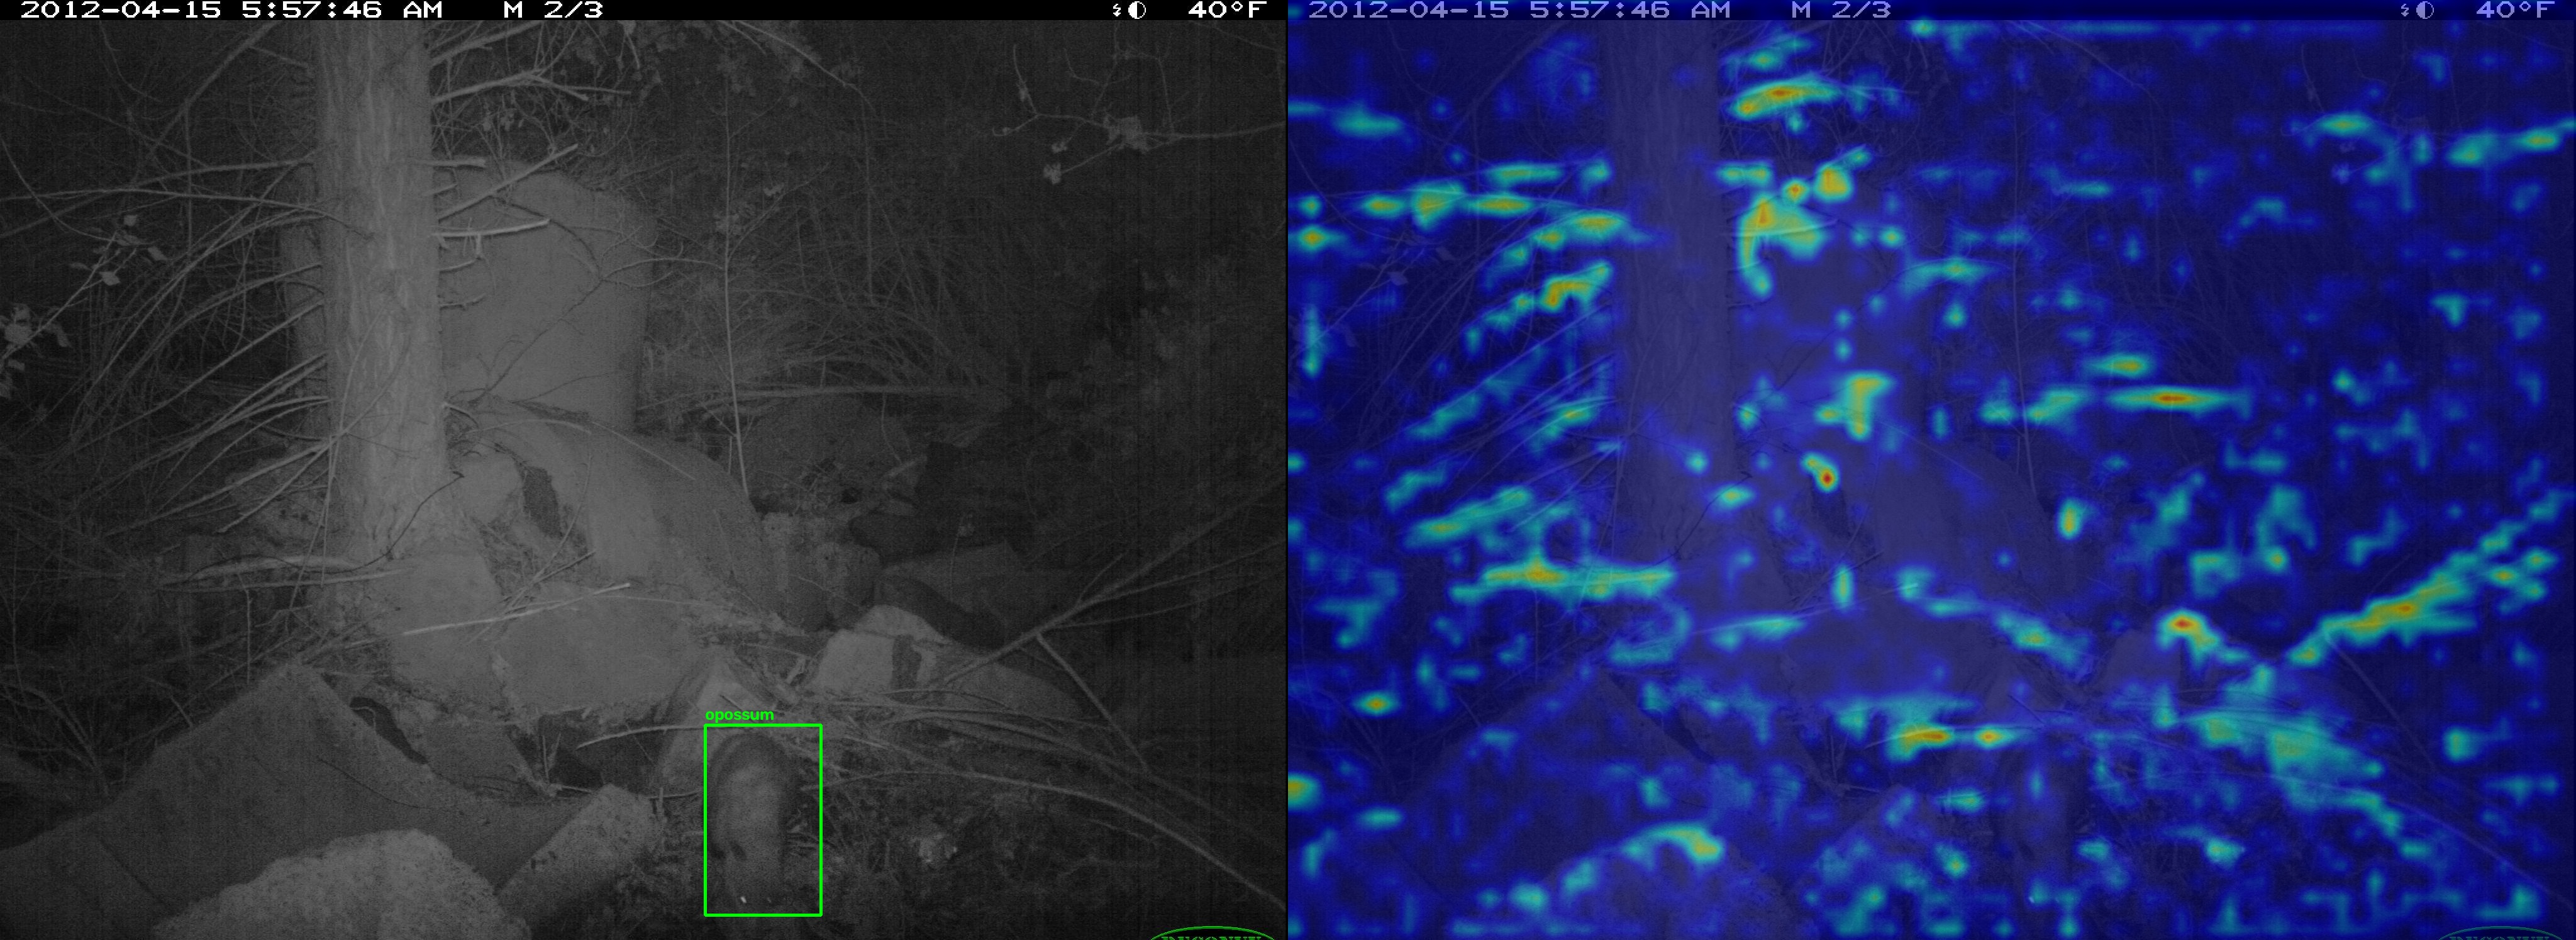
\includegraphics[width=0.5\textwidth]{figuras/trans_test_falso_positivo.jpg}
  \caption{Grad-CAM en una ubicación nunca vista. A la izquierda, la imagen con
    la caja anotada (un \texttt{opossum} al pie de las rocas, abajo al centro);
    a la derecha, el mapa de activación de la clase correcta. La evidencia se
    reparte por la vegetación, las ramas y las rocas de todo el cuadro y apenas
    toca al animal; el modelo no acertó ninguna detección. Es el caso que la
    razón de masa cuantifica: el mapa no está vacío, lo que activa no es el
    animal.}
  \label{fig:gradcam}
\end{figure}

El indicador es la \emph{razón de masa}: qué fracción de la activación cae
dentro de las cajas anotadas, dividida por el área que esas cajas ocupan. Vale
1.0 cuando el mapa es uniforme, es decir cuando el modelo no localiza nada.

Sobre 120 imágenes por partición, la mediana es 1.12 en \texttt{cis\_test} y
1.00 en \texttt{trans\_test}: en la mitad de las imágenes de
ubicaciones nuevas la evidencia del modelo no está más concentrada sobre el
animal que si estuviera repartida al azar. En 52 de 120 imágenes conocidas y 62
de 120 nuevas la razón no supera 1.0.

El desglose por tamaño es más específico y más incómodo. Para animales que
ocupan menos del 1\% del cuadro, la razón es 1.89 en ubicaciones conocidas y
0.89 en ubicaciones nuevas, por debajo de 1.0: la
activación está \emph{menos} concentrada sobre el animal que un mapa uniforme.
Para animales grandes apenas baja, de 1.43 a 1.27. La degradación de
localización se concentra exactamente donde el modelo ya era más débil, y es
coherente con lo que la Sección~\ref{sec:generalizacion} mide con el mAP: en una
cámara nueva, lo que sostenía la detección de un animal chico no estaba en el
animal. La Figura~\ref{fig:gradcam} muestra un caso concreto.

\subsection{Robustez ante tamaño y oclusión}
\label{sec:robustez}

\begin{table}[t]
  \centering
  \footnotesize
  \begin{tabular}{lllrr}
    \toprule
    Barrido & Partición & Nivel & Cajas / imág. & mAP@0.5 \\
    \midrule
    tamaño & \texttt{cis\_test} & diminuto$^{\dagger}$ (0.000--0.00) & 18 & 0.1602 \\
    tamaño & \texttt{cis\_test} & chico (0.002--0.01) & 891 & 0.5131 \\
    tamaño & \texttt{cis\_test} & mediano (0.010--0.05) & 8\,727 & 0.8033 \\
    tamaño & \texttt{cis\_test} & grande (0.050--1.01) & 3\,120 & 0.7341 \\
    tamaño & \texttt{trans\_test} & diminuto$^{\dagger}$ (0.000--0.00) & 16 & 0.0913 \\
    tamaño & \texttt{trans\_test} & chico (0.002--0.01) & 1\,719 & 0.2310 \\
    tamaño & \texttt{trans\_test} & mediano (0.010--0.05) & 11\,878 & 0.4555 \\
    tamaño & \texttt{trans\_test} & grande (0.050--1.01) & 4\,512 & 0.2852 \\
    oclusión & \texttt{cis\textbackslash\{\}\_test} & sin tapar & 1\,500 & 0.7652 \\
    oclusión & \texttt{cis\textbackslash\{\}\_test} & centro, 25\% & 1\,500 & 0.2375 \\
    oclusión & \texttt{cis\textbackslash\{\}\_test} & centro, 50\% & 1\,500 & 0.0584 \\
    oclusión & \texttt{cis\textbackslash\{\}\_test} & centro, 75\% & 1\,500 & 0.0044 \\
    oclusión & \texttt{cis\textbackslash\{\}\_test} & inferior, 25\% & 1\,500 & 0.3699 \\
    oclusión & \texttt{cis\textbackslash\{\}\_test} & inferior, 50\% & 1\,500 & 0.0647 \\
    oclusión & \texttt{cis\textbackslash\{\}\_test} & inferior, 75\% & 1\,500 & 0.0234 \\
    \bottomrule
  \end{tabular}
  \caption{Robustez ante tamaño del objeto y ante oclusión sintética. En el barrido de tamaño, una imagen entra en un tramo solo si \emph{todas} sus cajas caen en el rango —filtrando caja por caja, las descartadas seguirían en la imagen y cada detección correcta de un animal fuera del rango contaría como falso positivo; $^{\dagger}$ menos de 50 cajas. En el de oclusión, el parche tapa la fracción indicada del \emph{área} de cada caja anotada sobre una submuestra fija por semilla: \texttt{centro} deja la silueta y quita la textura, \texttt{inferior} tapa desde el borde de abajo, como la vegetación real, y rompe también la silueta.}
  \label{tab:robustez}
\end{table}


Las imágenes originales son $2048\times1494$ y entran a la red a 640 px, una
reducción de 3.2 veces. Un animal lejano, que ya ocupaba pocos píxeles, queda en
unos pocos. El barrido por tamaño cuantifica ese costo, el caso dominante del
dominio y no una situación marginal.

La oclusión es sintética porque el conjunto no trae esa anotación; la
alternativa era no responder el entregable. El parche tapa la fracción indicada
del \emph{área} de cada caja anotada, y los dos modos no miden lo mismo
(\texttt{centro} deja la silueta y quita la textura; \texttt{inferior} la tapa
desde abajo, como la vegetación real). La interpretación es limpia porque, como
se verificó en la Sección~\ref{sec:metodo_aumento}, el modelo nunca vio oclusión
durante el entrenamiento.

\subsection{Reporte de actividad ecológica}

El entregable \#5 pide demostrar el módulo sobre una cámara no vista en el
entrenamiento, el caso de despliegue real. La demostración principal es por eso
sobre \texttt{trans\_test} (9 cámaras nunca vistas, 2\,090 noches-cámara), con
\texttt{cis\_test} al lado como caso favorable. Las 18\,846 detecciones por
encima de 0.25 se agrupan en 6\,637 eventos independientes (ventana de 30
minutos) contra 4\,819 de las cajas anotadas; en \texttt{cis\_test} son 13\,559
detecciones y 3\,706 eventos. Contar detecciones en vez de eventos habría
inflado la actividad, porque las cámaras disparan ráfagas.

\begin{table}[t]
  \centering
  \footnotesize
  \begin{tabular}{lrrr|rrr}
    \toprule
    Especie & Eventos & Error & Noct. & Eventos & Error & Noct. \\
    \midrule
    \texttt{opossum} & 1\,302 & +14\% & 73\% & 750 & +2\% & 80\% \\
    \texttt{raccoon} & 1\,016 & +15\% & 70\% & 410 & +74\% & 77\% \\
    \texttt{cat} & 786 & +234\% & 46\% & 360 & +21\% & 35\% \\
    \texttt{coyote} & 724 & +30\% & 58\% & 564 & +17\% & 51\% \\
    \texttt{car} & 679 & +12\% & 4\% & 319 & +2\% & 8\% \\
    \texttt{bobcat} & 655 & +13\% & 52\% & 342 & +32\% & 49\% \\
    \texttt{rabbit} & 403 & +108\% & 28\% & 310 & +24\% & 24\% \\
    \texttt{dog} & 309 & +74\% & 7\% & 192 & +42\% & 11\% \\
    \texttt{squirrel} & 252 & +6\% & 2\% & 154 & +18\% & 0\% \\
    \texttt{bird} & 244 & +281\% & 20\% & 139 & +45\% & 12\% \\
    \texttt{skunk} & 226 & +81\% & 71\% & 87 & +12\% & 66\% \\
    \texttt{rodent} & 25 & +150\% & 60\% & 41 & +5\% & 88\% \\
    \texttt{fox} & 9 & +800\% & 89\% & 4 & +100\% & 75\% \\
    \texttt{deer} & 5 & --- & 0\% & 34 & +26\% & 50\% \\
    \texttt{badger} & 2 & -75\% & 100\% & --- & --- & --- \\
    \bottomrule
  \end{tabular}
  \caption{Reporte de actividad por especie. A la izquierda la demostración principal, cámaras nunca vistas (\texttt{trans\_test}: 9 cámaras, 2\,090 noches-cámara); a la derecha el caso favorable, cámaras vistas en el entrenamiento (\texttt{cis\_test}: 10 cámaras, 1\,131 noches-cámara). Un evento independiente agrupa detecciones de la misma especie y cámara separadas por menos de 30 minutos. `Error' es la diferencia relativa de los eventos del modelo contra el mismo reporte calculado desde las cajas anotadas a mano: es la validación del módulo, no un adorno. `Noct.' es el índice de nocturnidad, un control contra la historia natural conocida de cada especie.}
  \label{tab:actividad}
\end{table}


El índice de nocturnidad reproduce la historia natural conocida de las especies
aun en cámaras nuevas, sin recibir esa información: 2\% para \texttt{squirrel},
20\% para \texttt{bird} y 4\% para \texttt{car} (diurnos); 73\% para
\texttt{opossum}, 70\% para \texttt{raccoon} y 71\% para \texttt{skunk}
(nocturnos); 58\% para \texttt{coyote} y 52\% para \texttt{bobcat}
(crepusculares). Es un control que cuesta una columna y detecta errores que el
mAP no ve.

El error contra las anotaciones es lo que decide para qué sirve el módulo. En
\texttt{cis\_test} es siempre positivo y chico, de $+2\%$ a $+100\%$, con las
especies de más datos cerca del valor real (\texttt{opossum} $+2\%$, \texttt{car}
$+2\%$) y las intermedias disparadas (\texttt{raccoon} $+74\%$). En
\texttt{trans\_test} crece (\texttt{cat} $+234\%$, \texttt{bird} $+281\%$) y, a
diferencia de las cámaras conocidas, va en las dos direcciones: \texttt{deer},
sin ninguna caja anotada en esa partición, recibe cinco eventos inventados,
mientras \texttt{badger} se subestima ($-75\%$: ocho eventos anotados, dos
detectados), la especie rara perdida justo donde más importaría registrarla. Esa
tabla de error es el número que un reporte automático debe entregar junto con sus
conclusiones.
